%!TEX root = ../thesis.tex

%%%%% Chapter: Software Setup %%%%%
\chapter{Software Setup}

\ifpdf
    \graphicspath{{Chapter8/Figs/Raster/}{Chapter8/Figs/PDF/}{Chapter8/Figs/}}
\else
    \graphicspath{{Chapter8/Figs/Vector/}{Chapter8/Figs/}}
\fi


\section{Overview}

\DTsetlength{0.2em}{6em}{0.2em}{0.7pt}{2.3pt}

A simplified directory tree of the source code is shown below:

\dirtree{%
.1 root/.
.2 system/.
.3 aux/.
.3 elements/.
.3 subsystems/.
.2 eval/.
.3 align.py.
.3 ocr.py.
.2 gui/.
.3 root.py.
.3 system.py.
.3 labeller.py.
}

The \texttt{system/} folder contains the fundamental setups including the implementations of all the subsystems (OCR, Speech Recogniser, Alignment Algorithm), all the basic elements explained in \Cref{chap:basic-elem} and some auxilliary functions like the \texttt{diff} with JWF input. The \texttt{eval/} folder contains functions to compute all the evaluation metrics described in \Cref{chap:eval-framework}. The \texttt{gui/} folder visualises the main functionalities implemented in the \texttt{system/} and \texttt{eval/} folders.

\section{The \texttt{system/} Folder}

The \texttt{system/} folder implements the core parts of the system architecture, which forms the basis of the entire software setup. The \texttt{system/} folder contains 3 main child folders: \texttt{subsystems/}, \texttt{elements/} and \texttt{aux/}.

\subsection{The \texttt{subsystems/} child folder}

The \texttt{subsystems/} child folder contains the implementations (or wrappers) of the Tesseract OCR engine, Google Cloud Speech Recogniser and the \texttt{diff}-based alignment algorithm, as 3 separate Python (\texttt{.py}) files (not shown in the directory tree for simplicity).

The Tesseract OCR is integrated into the system using the \texttt{pytesseract} wrapper, and the engine can run locally without Internet connection. The Google Cloud Speech-to-Text service also has Python APIs, but it requires stable Internet connection to send requests and receive the transcription results. The Google Cloud also needs my personal credentials before the speech-to-text service can actually be used in the system.

The \texttt{diff}-based alignment algorithm is based on the self-implemented JWF-based alignment algorithm stored in the \texttt{aux/} folder. It first obtain the optimal alignment based on the parameterised JWF function defined in \Cref{eq:jwf-final}, and then return the final alignment result as a \texttt{Matches} object using the method explained in \Cref{sec:align-in-system}.

\subsection{The \texttt{elements/} child folder}

This child folder contains all the implementations of the basic elements defined in \Cref{chap:basic-elem}. This folder is a core dependency for almost all other files, especially for the files in the \texttt{system/} and the \texttt{eval/} folder.

\subsection{The \texttt{aux/} child folder}

This child folder includes the helper functions used by the system. We have mentioned earlier that this folder contains an important implementation which solves the optimal alignment of two sequences with a configurable JWF input. The actual implementation of finding the optimal alignment uses the Hirschberg's algorithm \cite{hirschberg1975linear}, which can achieve linear space complexity by a clever modification of the Needleman-Wunsch Algorithm (mentioned in \Cref{sec:diff-formulation}).


\section{The \texttt{eval/} Folder}

The \texttt{eval/} folder contains two main files \texttt{ocr.py} and \texttt{align.py}, which implement the evaluation functions for the Tesseract OCR and the alignment algorithm respectively. These evaluation functions highly rely on the basic elements and their associated operations defined in \texttt{system/elements/}. For instance, the intersection area between two \texttt{BBoxGroup} objects \texttt{a} and \texttt{b} could be calculated using the simple expression \texttt{(a \& b)}, which is heavily used in the evaluation of OCR output bounding-boxes.


\section{The \texttt{gui/} Folder}

The GUI implementation visualises the core components in the system, including the system parameter control, final system output and the system evaluation results. The GUI implementation is based on the Tkinter module, which is the Python binding to the Tk GUI Toolkit. It allows the users to easily interact with the core system (implemented in \texttt{gui/system.py}), and also allows the system developers (like me) to label the ground-truth dataset for the purpose of evaluation (implemented in \texttt{gui/labeller.py}). The GUI can be initiated by running \texttt{gui/root.py}.

\subsection{\texttt{gui/system.py}}

\begin{figure}[!ht]
    \centering
    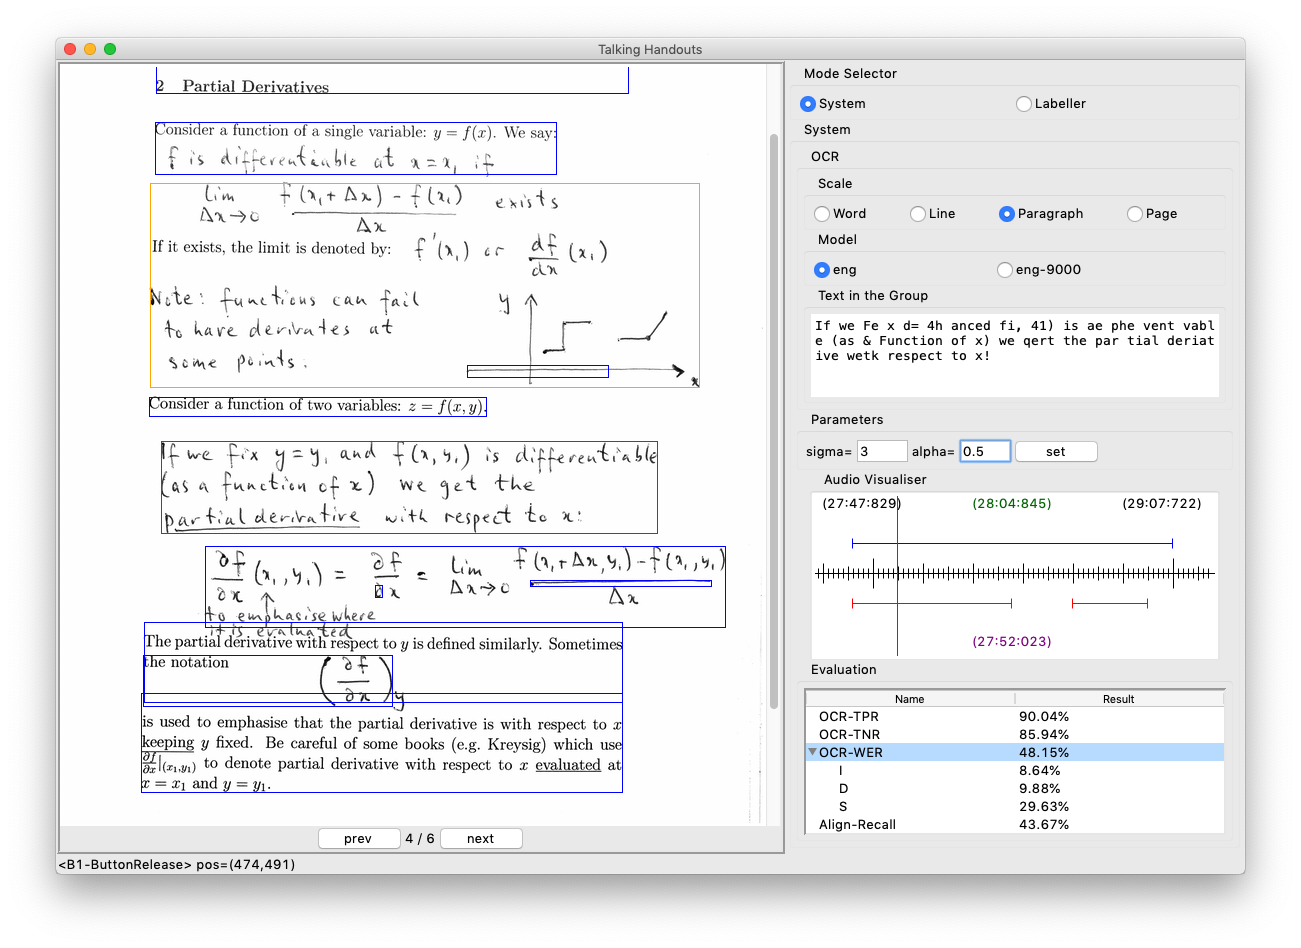
\includegraphics[width=\textwidth]{gui-system.png}
    \caption{The `System' mode of the GUI}
    \label{fig:gui-system}
\end{figure}

\Cref{fig:gui-system} shows a screenshot of the `system' mode of the GUI. The users are able to select between the 4 OCR scales, 2 OCR models (\texttt{eng} and \texttt{eng-9000}) and they could also adjust the parameters $\sigma_t$ and $\alpha_c$ for the alignment algorithm. The resulting bounding-boxes are rendered in the left, and the corresponding alignment output audio segments (in blue) and the assigned ground-truth segments (in red) are shown in the audio visualiser to the right.

Users can click any bounding-box in the left and listen to the lecture audio by clicking a specific position in the audio visualiser. The audio playback can be stopped by pressing spacebar. 

The evaluation results are also listed in the bottom-right corner. The evaluation results in \Cref{chap:eval-results} are logged from this GUI listing.

\subsection{\texttt{gui/labeller.py}}

\begin{figure}[!ht]
    \centering
    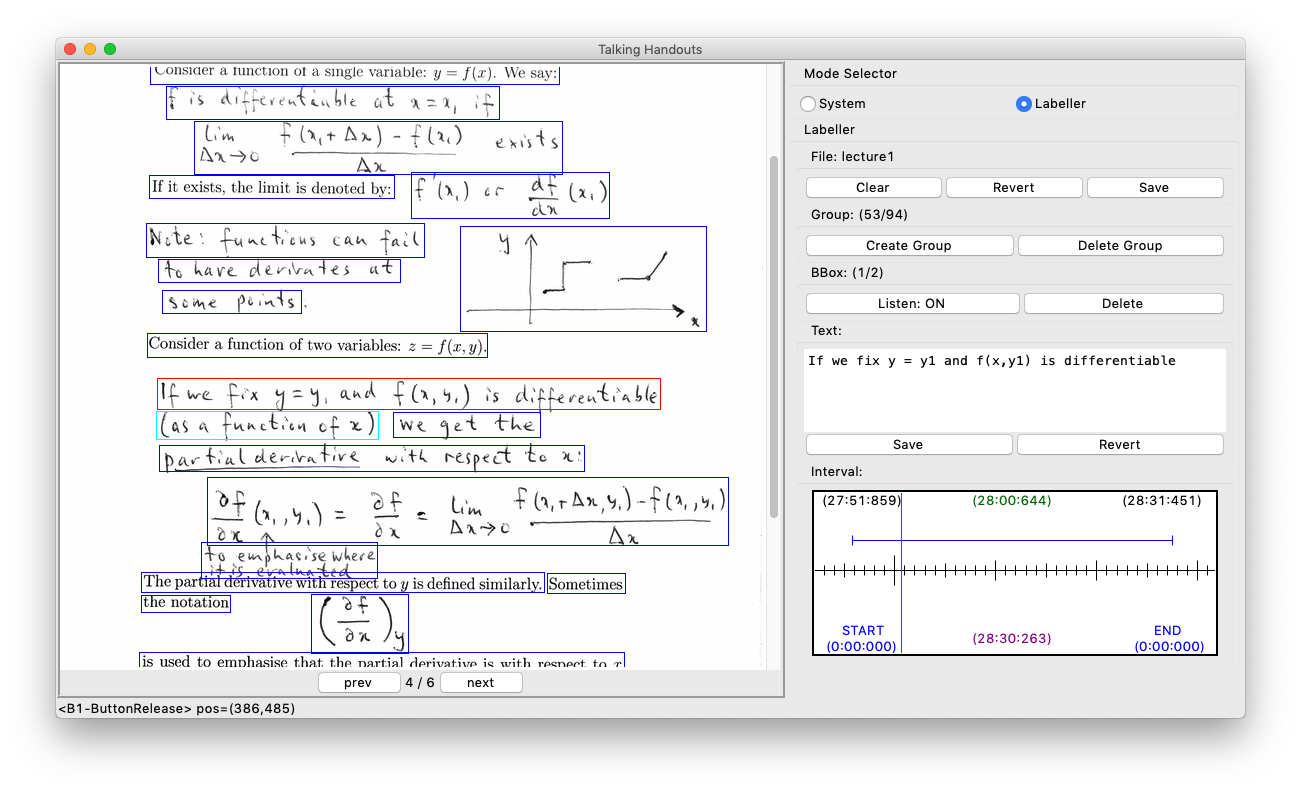
\includegraphics[width=.9\textwidth]{gui-labeller.png}
    \caption{The `Labeller' mode of the GUI}
    \label{fig:gui-labeller}
\end{figure}

The `labeller' mode is implemented for the purpose of labelling ground-truth data for the evaluation framework. A new \texttt{BBoxGroup} object can be created by clicking `Create Group' and \texttt{BBox} objects can be added to this group by drawing rectangles directly in the left on the handouts. The reference text for each \texttt{BBox} should be typed in the textbox above the audio visualiser. For each labelled \texttt{BBoxGroup}, the corresponding audio segments can also be labelled in the audio visualiser on the right.